% Template for ICASSP-2019 paper; to be used with:
%          spconf.sty  - ICASSP/ICIP LaTeX style file, and
%          IEEEbib.bst - IEEE bibliography style file.
% --------------------------------------------------------------------------
\documentclass{article}
\usepackage{spconf,amsmath,graphicx}
\usepackage{booktabs}
%...
% Example definitions.
% --------------------
\def\x{{\mathbf x}}
\def\L{{\cal L}}

 \graphicspath{{figs/}}
% Title.
% ------
\title{Noise reduction by resynthesizing with vocoder}
%
% Single address.
% ---------------
\name{Author(s) Name(s)\thanks{Thanks to XYZ agency for funding.}}
\address{Author Affiliation(s)}
%
% For example:
% ------------
%\address{School\\
%	Department\\
%	Address}
%
% Two addresses (uncomment and modify for two-address case).
% ----------------------------------------------------------
%\twoauthors
%  {A. Author-one, B. Author-two\sthanks{Thanks to XYZ agency for funding.}}
%	{School A-B\\
%	Department A-B\\
%	Address A-B}
%  {C. Author-three, D. Author-four\sthanks{The fourth author performed the work
%	while at ...}}
%	{School C-D\\
%	Department C-D\\
%	Address C-D}
%
\begin{document}
%\ninept
%
\maketitle
%
\begin{abstract}

\end{abstract}
%
\begin{keywords}
%One, two, three, four, five
\end{keywords}
%

\section{Introduction}
\label{sec:intro}
General approach of speech enhancement systems are to modify the original signal to make it more like the clean signal. These systems suffer from the problem of over-suppression of signal and under-suppression of noise.   Ideally, speech enhancement systems should remove noise completely without hampering the speech quality. Alternatively speech synthesis systems can produce high-quality speech from text. Such systems are able to learn the mapping of text to acoustic parameters of the speech signal, where the speaker is uttering the text. 
%In the paper \cite{chen2006new} author

Traditional speech synthesis systems are of two types, concatenative: where small speech chunks are stitched together to generate speech and parametric: where a model is used to learn the mapping of text to acoustic parameters of speech  and from the acoustic parameter generate speech by using a vocoder. Concatenative models are speaker dependent and generally large dictionary is required. Parametric models are more flexible, as you only need to train the model to predict acoustic features from text and this mapping is speaker independent. They are limited in terms of vocoder, as vocoder speech is generally reported less natural to concatenative synthesis models. 

Speech enhancement uses noisy speech as input, Noisy speech signal has more information about the clean speech signal than simple text. Noisy signal has also information about prosody which is difficult to generate with TTS. Hence, we can build a system that takes noisy audio as input and learns the mapping to acoustic parameters of clean speech. Next from the acoustic parameters we can generate clean speech using a vocoder. We train a neural network based model to learn the mapping of clean speech vocoder parameters from noisy speech. The hypothesis here is that modifying the original signal can result in signal distortion. We can achieve better quality by synthesizing a cleaner version of the noisy signal. 

In this paper, we first train a TTS system using cmu arctic dataset. We take a Text-To-Speech (TTS) framework merlin \cite{wu2016merlin} to synthesize audio from text. Next we train a prediction model to learn acoustic parameters from noisy speech. Then, we synthesize new audio signal from noisy speech. We add four environmental noise from Blizzard \cite{KingAndKaraiskos2013} to clean speech to create the noisy speech. We evaluate the prediction errors in acoustic parameter with objective evaluation. Next we evaluate the intelligibility and quality  of the resynthesized speech  and compare it with a mask based system and wiener filter. We show that the model generates speech that is noise-free and high quality than Wiener filter. We also show that generated speech intelligibility is comparable with wiener filter. We also test that out model is speaker-dependent by evaluating with two speakers together and individually.



\section{Background Research}
\label{sec:back}
In recent years the

%%%%%%%%%%%%%%%%%%%%%%%%%%%%%%%%%%%%%%%%%%%%%%%%%%%%%%%%%%%%%%%%%%%%
\section{Model Overview }
\label{sec:mod_ovr}
Traditional statistical TTS system can generate speech from text. In a simplified view, TTS systems consist of two stages, first where with speech and corresponding text acoustic model is trained to map text to acoustic features of the speech. Instead of using text, mapping is learned from linguistic specification.  The second stage is to synthesize speech from acoustic features using a vocoder.

Our vocoder denoising system follows the same stages. In the training part, a prediction model is trained with noisy speech and corresponding clean speech. The prediction model learns to generate the acoustic features of clean speech from a noisy signal. We use a neural network for the prediction model. In the synthesis part, new signal is generated from acoustic features using a vocoder. 

\begin{figure*}[htb]
\begin{minipage}[b]{0.9\linewidth}
  \centering
  \centerline{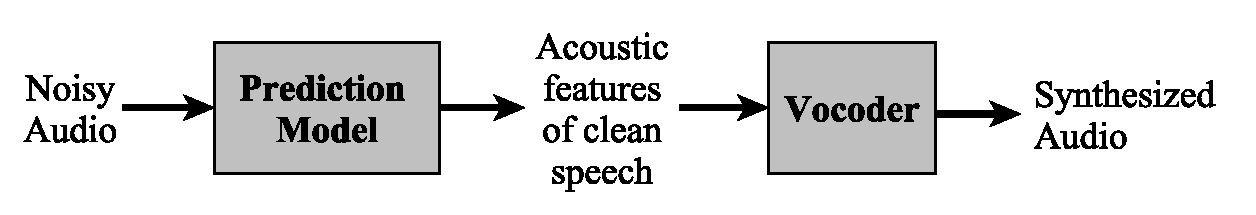
\includegraphics[width=0.95\textwidth]{model.eps}}
%  \vspace{2.0cm}
%  \centerline{(a) Result 1}\medskip
\end{minipage}
\caption{Vocoder denoising model}
\label{fig:res}
\end{figure*}

\subsection{Relation to speech synthesis}
\label{sub:speech_synth}

Statistical speech synthesis systems synthesize audio from text using vocoders. Traditional statistical speech synthesis models has two ends, front end that produces linguistic specification from text and back-end, that predicts acoustic features from linguistic specifications. Our acoustic feature model is similar to the back-end of such systems. We first train prediction model with noisy audio features as input and clean acoustic features as output. In second stage, we predict acoustic features from the noisy audio.  Third and last stage of the model is to resynthesize audio with vocoder from the predicted acoustic features. We use speech synthesis Merlin toolkit \cite{wu2016merlin} for implementation of the model. We believe there is more information in noisy audio about the acoustic features of clean audio signal than text, so we can create a clean resynthesis from noisy signal that can be better intelligibilty and quality than TTS system. The resynthesis would be clean, and hence will give better noise suppression performance.

\subsection{Synthesizing speech from acoustic features}
\label{sub:voc_feat}
We use a vocoder to generate clean resynthesis of the noisy speech. The vocoder is traditionally used to generate a compact representation of audio, so that audio can be transmitted with less information. It consists of two parts, encoder, that converts speech to compact representation and decoder, that receives the representation and generates speech waveform. Here, the compact representation are set of acoustic features. This set up is also used in STTS systems. 

Three acoustic parameters are used, spectral envelope,  fundamental frequency ($F0$) and aperiodic energy of spectral envelope. Fundamental frequency can be used to predict voicing decision which is another parameter required for vocoder. 

\subsection{Prediction Model}
\label{ssec:model}
The prediction model takes noisy signal spectrum as input and predicts the acoustic features of clean speech. The output features are extracted with encoder part of vocoder. Vocoder acoustic features are predicted from the signal at a fixed frame rate. We first used a feed-forward DNN with 4 layers. Each layer has 512 neurons and tanh activation function. As input we use, log mel-spectrogram of the noisy frame with neighboring frames ($\pm 4$). The output layer of prediction model consist of raw vocoder features with their first and second derivative concatenated. This approach again following STTS synthesis models. Next we tried a sequence LSTM model with 2 layers, as input only one frame is used now.

\subsection{Evaluation}
\label{sec:evaluation}
We wvaluate the synthesized speech in two parts. First part evaluating the performance of prediction model. For the first two vocoder parameters (spectral envelope and band aperiodicity), We can measure distortion between predicted and ground truth. Distortion should be less for better models. To measure accuracy with fundamental frequency, two measures are used, root mean square error and Pearson's correlation between ground truth and prediction and classification error is measured for voiced/unvoiced flag. 

The second part is evaluating the clean resyntheis of vocoder denoising system.
The third part is evaluating vocoder limitations. Vocoded speech can sound mechanical or muffled at times. So we run vocoder encoder and decoder on clean speech to generate vocoded clean speech. We use this files in listening tests to measure vocoder loss. We use WORLD vocoder for all out experiments.

\section{Experiments}
\label{sec:expr}

\subsection{Dataset}
\label{ssec:data}
Noisy dataset is generated from adding environmental noise to a speech dataset. For speech data, we use CMU arctic dataset \cite{kominek2004cmu}. The arctic dataset contains clean recorded speech from different speakers. The sentences are taken from different parts of project gutenberg, with 1132 sentences in total. To make the data noisy, we add environmental noise from Blizzard 2013 challenge \cite{KingAndKaraiskos2013}. Four types of noises are present in the dataset, street, pedestrian, cafe and bus noise. Six channels are available for each noisy file, we treat all channels as separate noise source. We mix clean speech with one of the random noise files starting from random offset with constant gain of 0.95. The SNR of noisy files ranges from 21 dB to -6 dB, with average 6 dB. The sentences are 2 to 13 words long, with mean length of 9 words. We use female speech corpus (slt) for all experiments, male (bdl) voice is also used to test speaker dependency of the system. Dataset is partitioned to 1000-66-66 as train-dev-test. 
 
We use WORLD vocoder \cite{morise2016world}, which is open source and available with merlin toolkit. Input and output features are extracted with window size of 1024 at fixed 5 ms frame rate. Log mel spectrogram is extracted from noisy audio and used as input features for prediction model. Output feature labels (spectral envelope, band aperiodicity and F0) are generated from WORLD.


%%%%%%%%%%%%%%%%%%%%%%%%%%%%%%%%%%%%%%%%%%%%%%%%%%%%%%%%%%%%%%%%%%%%%%%%%%%%%%%%%%%%%%%%%%%%%%

\subsection{TTS Objective measures}
Mel cepstral distortion (MCD), band aperiodicity
distortion (BAPD), and root mean square error of F0 (RMSE),
Pearson correlation F0 (Corr.) and voiced/unvoiced error rate.

\begin{table*}[hbt]
    \centering
    \begin{tabular}{ccccccc} \toprule
     & \multicolumn{2} {c} {\bfseries Spectral Distortion } & \phantom{abc} & \multicolumn{3} {c} {\bfseries $F0$ measures} \\ 
     \cmidrule{2-3}  \cmidrule{5-7}
     System                     & MCD (dB) & BAPD (dB) && RMSE (Hz) & CORR & UUV \\ 
    \midrule
    TTS (DNN)                   & 5.28  & 0.25       && 13.064   & 0.71 & 6.66\% \\
    TTS (LSTM)                  & 5.05  & 0.24       && 12.60    & 0.73 & 5.60\% \\
    estimated\_from\_clean      & 2.68  & 0.16      && 4.95 & 0.964 & 2.78\% \\
    estimated\_from\_noisy (DNN)  & 5.07 & 0.19     && 8.83 & 0.93 & 6.48\% \\
    estimated\_from\_noisy (LSTM) & 4.81 & 0.19     && 5.62 & 0.95 & 5.27\% \\
    \bottomrule
    \end{tabular}
    \caption{TTS objective measures: MCD,BAPD,RMSE,VUV lower is better, CORR higher is better.}
    \label{tab:obj_eval_tts}
\end{table*}


%%%%%%%%%%%%%%%%%%%%%%%%%%%%%%%%%%%%%%%%%%%%%%%%%%%%%%%%%%%%%%%%%%%%
\subsection{Evaluating Speaker dependency}
\begin{table*}[hbt]
    \centering
    \begin{tabular}{cccccccc} \toprule
& & \multicolumn{2}{c}{\bfseries Spectral Distortion} & \phantom{abc}& \multicolumn{3}{c}{\bfseries $F0$ measures}\\
\cmidrule{3-4}  \cmidrule{6-8}
    Speaker & \#sentences & MCD & BAPD && RMSE & CORR & UUV \\
     \midrule
    Female (slt)    & 1132 & 4.81 & 0.19 && 5.62  & 0.95 & 5.27\% \\
    Male (bdl)      & 1132 & 5.49 & 0.22 && 10.33 & 0.84 & 12.53\%\\
    Both (slt+bdl)  & 2264 & 4.96 & 0.20 && 9.22  & 0.96 & 8.89\%\\ \bottomrule
    \end{tabular}
    \caption{Estimation errors in different speakers}
    \label{tab:speaker}
\end{table*}

%%%%%%%%%%%%%%%%%%%%%%%%%%%%%%%%%%%%%%%%%%%%%%%%%%%%%%%%%%%%%%%%%%%%
\subsection{Evaluating vocoder denoising system}

\begin{table}[hbt]
    \centering
\begin{tabular}{ccc}
\toprule
Model & PESQ & STOI \\
\midrule
Clean               & 4.50 & 1.00 \\
Noisy               & 1.88 & 0.88\\
IRM                 & 2.26 & 0.80\\
Wiener              & 2.26 & 0.88 \\
Estimate            & 2.43 & 0.87 \\
Vocoder\_enc\_dec   & 3.39 & 0.93 \\
Estimate\_clean     & 2.98 & 0.92\\
TTS                 & 1.33 & 0.08\\
\bottomrule
\end{tabular}
\caption{ Objective Intelligibility (STOI) and Quality (PESQ)}
\label{tab:obj_denoise}
\end{table}






\begin{figure}[htb]
\begin{minipage}[b]{1.0\linewidth}
  \centering
  \centerline{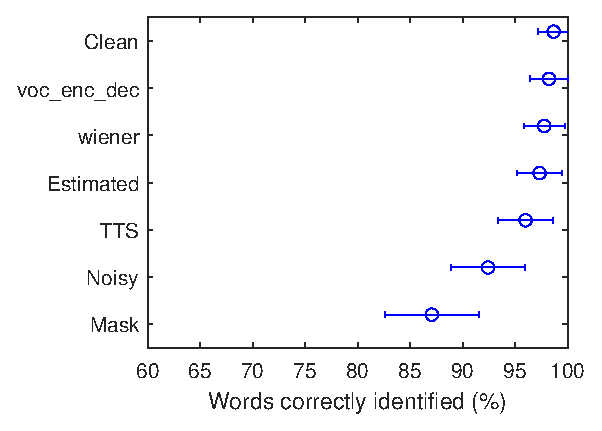
\includegraphics[width=.9\linewidth]{00-intel.eps}}
%  \vspace{1.5cm}
  \centerline{(b) Subjective intelligibility results over 2 subjects}\medskip
\end{minipage}
%
\begin{minipage}[b]{1.0\linewidth}
  \centering
  \centerline{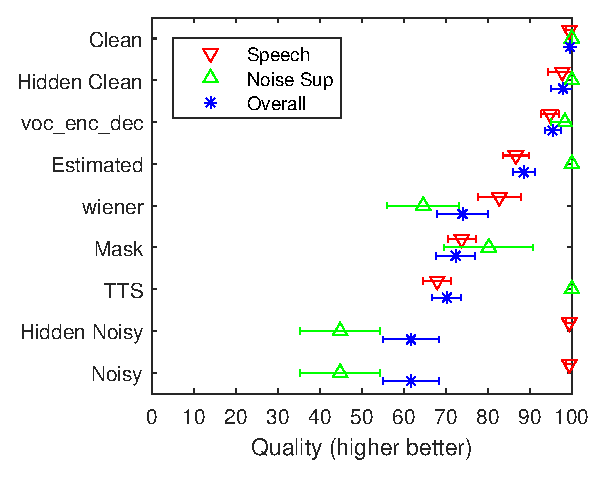
\includegraphics[width=.92\textwidth]{01-qual.eps}}
%  \vspace{1.5cm}
  \centerline{(c) Subjective quality results over 2 subjects}\medskip
\end{minipage}
\caption{Listening test results}
\label{fig:res}
%
\end{figure}
\vfill\pagebreak



\section{REFERENCES}
\label{sec:refs}

% References should be produced using the bibtex program from suitable
% BiBTeX files (here: strings, refs, manuals). The IEEEbib.bst bibliography
% style file from IEEE produces unsorted bibliography list.
% -------------------------------------------------------------------------
\bibliographystyle{IEEEbib}
\bibliography{strings,refs}

\end{document}
